\chapter{Results and Discussion}
{\label {chapter3}}
In chapter 2, we introduced a method that smoothly interpolates between multiple topological
states to obtain a smooth potential surface. This method is general and adaptive and requires
only one input parameter, and that is the location of the region where the topological change
occurs. In non-adiabatic dynamics literature, this region is called seam\footnote{The term
seam is used throughout the rest of this document and it should be emphasized that although
in one-dimensional potentials this the region is just a point but in higher dimensional
potential surfaces, seam may be a multi-dimensional surface. We use this term to keep the
complete meaning of the hopping region in general cases.}. There are two main
applications for this method that we may envision: (a) computing
potential energy surfaces for quantum nuclear dynamics and reaction coordinate dependent
potential surfaces,(b) classical molecular dynamics simulation. While the seam may be known
during classical molecular dynamics simulations, such information may not be readily
available when multidimensional potential surfaces are to be computed. This is because such
surfaces need repeatedly large number of electronic structure calculations and some kind of
sampling procedure may be utilized to reduce the number of such calculations, thereby skipping
the seam. Hence one critical question that arises in the algorithm mentioned above is how
precisely does the seam need to be known and in this chapter we present benchmarks
that indicate that this information is not necessary to be known in an extremely precise
fashion. In fact, our tests here show that where errors in detection of the seam
is of the order of 0.3 \AA, potential surfaces are still quite accurate.




The above discussion is an algorithmic matter though, and the question remains as to the
 kind of chemical problems that are most affected by such a scheme. Reactive systems with
localized changes in topology may always be handled through appropriate choice of fragments
that exploit chemical intuition. But hydrogen bonded systems and weakly bound networks can
exhibit changes in configuration that require multiple topologies that are sometimes
impossible to predict a priori. A few problems that characterize such events are :
(a) solvation of molecules and peptides in a cluster of water,(b) solution of ions such
as excess proton and OH- in water that relate to acid base chemistry and are also seen in
protonic conducting systems and fuel cells, and (c) biological & biologically inspired
ion-channels. In this chapter we consider protonated water clusters of various sizes and
gauge the accuracy of the method discussed in the previous chapter in computing accurate
potentials. Future work involves the development of this procedure into a robust tool to
compute multidimensional potentials by coupling the method to recently developed sampling
techniques \cite{sumner2007quantum, jakowski2006computational, li2014vibrational,
hocker2011shannon, shannonIsoprene}. Funneling from this a multitopology Hamiltonian
formalism is also discussion in chapter 4.

\section{Protonated water clusters and wires}
{\label{intoToTestSystems}}
Proton transport through water is an important problem due to its wide range of applications in
areas such as biology, atmospheric, and condensed phase chemistry \cite{fragAIMD-elbo}. Several
methods \cite{lobaugh1996quantum, tuckerman1995ab, tuckerman1994ab, schmidt1997molecular,
billeter1998protonizable, vuilleumier1997molecular, vuilleumier1998extended, vuilleumier1998quantum,
vuilleumier1999transport, schmitt1998multistate} have been developed to simulate the transport of
excess proton through water molecules. This excess charge of proton is delocalized over a few hydrogen
bonds. It has also been well known that Zundel ($H_5O_2^+$) and Eigen ($H_9O_4^+$) are two main
forms of hydrated proton structures that exist in bulk water. Eigen cation has been shown to be more
stable than solvated zundel cation \cite{schmitt1999computer}. Protonated water is also known to
exist as chain of molecules in many constrained environments such as biological membranes,
carbon nanotubes \cite{dellago2003proton, mann2003water, cao2010mechanism}, ion channels and fuel
cells etc. The conduction of protons through biological
membranes is very different from other ions through them \cite{Roux}. It has been shown that the
rate of proton transport is 8 times faster than the water molecules passing through the membrane
\cite{pomesRoux1}. This is the reason that a proton hopping mechanism through a ``connected'' line
of water molecules called a water-wire or proton wire \cite{nagle1978molecular} is hypothesized to
exist inside the ion channel. Water-wire's enhanced proton transport rate has been confirmed with
different widths of ion channels as compared to the bulk water. Other than membranes or ion
channels, water-wires have also been shown to exist in the photosynthetic reaction center of
Rhodobacter sphaeroides \cite{baciou1995interruption}.

As described in Chapter 1, the requirement of AIMD in these reactive systems is computationally
expensive. Hence due to the intrinsic scaling of electronic structure, we utilize fragment based
method to reduce the computational cost. But proton transport causes topology changes during dynamics.
This makes systems involving proton transport good test systems for CTM method. These molecular
systems also show quantum nuclear effects such as hydrogen nuclear tunneling
during the proton transfer step. A reduced dimensional study of potential energy surfaces is
required to quantify the quantum nuclear effects. Again, due to the bottleneck of system size
in electronic structure calculations, we turn towards fragment based methods to obtain the potential
surfaces. Topology changes also occur during these fragment based potential energy surfaces
calculations. These topology changes need to be resolved to get a good accuracy of potentials.
Hence, CTM interpolation should be tested for both the dynamics and for the potential
surfaces.

We utilize Eigen system and three protonated water-wires $(H_2O)_{12}H^+$, $(H_2O)_{5}H^+$, and
$(H_2O)_{3}H^+$ as benchmark systems for potential energy surface calculations.
Fragmentation of all the protonated water clusters is done is such as way that primary fragments are
chosen to be water dimers or $H_5O_2^+$ and their overlaps as Hydronium ($H_3O^+$) or water.

Next we discuss on how to get these primary and derivative fragments for every geometry
during dynamics or potential scans. We need to come up with an adaptive topology detection scheme
which can give us topology for any given geometry. A brief discussion about two different schemes
is given in the next section.

\section{Adaptive detection of changes in topological networks}
{\label{autosubDiscussion}}
In the fragmentation based electronic structure program, PIE-ONIOM
\cite{fragAIMD}, one can automatically generate topologies for
protonated water clusters. Say, $O_{i}$ is an oxygen atom in a water cluster,
and $D_{i}$ represents its minimum oxygen-oxygen distance. A solvation
sphere containing a maximum of three additional water molecular is created
around each oxygen atom, such that the respective oxygen-oxygen distances
are $10\%$ off $D_{i}$. These oxygen atoms and the hydrogens within $1.4$
\AA ~from them are included to form primitive fragments. All fragments
containing excess proton in them are given a net charge of +1 and rest as
0. Fragments not containing any electrons, e.g. $H^{+}$ are excluded from
the calculations.

A more sophisticated approach to create fragments that is applicable to more
general systems beyond the water-clusters described above is by using Delaunay
triangulation. For a given set of points in a d-dimensional space, Delaunay
triangulation is a triangulation such that no point in lies inside the
circum-hypersphere of any d-simplex created after triangulation
\cite{delaunayOriginalPaper, cgalLibrary}. In simpler terms, for our molecular
systems, the coarse grained nodes (which are our set of points) are in a
3-dimensional space (d=3) and hence the corresponding circum-hyperphere is a
sphere and 3-simplex is a tetrahedron. This means that the whole molecular region
will be divided into different tetrahedons as shown in figure
\ref{dirichlet-tessalation}(b). None of the nodes will lie inside any of the
tetrahedrons. Similarly, for a set of points in 2-dimensional space (d=2), the
corresponding circum-hypersphere would be a circle and 2-simplex would be a
triangle.

Anyone of these approaches mentioned above are to be utilized to come up with a
fragmentation topology during each electronic structure calculation performed in
AIMD or in a potential scan. Fragmentation topology matrices in the neighbouring
steps need to be compared to see if the topology has changed. One of the ways to
do that is to just check the difference between the two matrices and see if that
is a zero or a non-zero matrix. If it is a non-zero matrix that means that the
fragmentation topology has changed in this step. Although it has been observed
that for the choice of first approach, the columns of fragmentation topology
matrix may permute during dynamics. This leads to the same set of primary as
well as derivative fragments but the difference between the two neighbouring
matrices turns out to be a non-zero matrix. This is why, a property of rectangular
matrices which is invariant under row/column permutations, should be compared
between the neighbouring fragmentation topology matrices. Singular value
decomposition (SVD) of matrices is one of these properties which are invariant
under row/column permutations. Difference of the vectors of n ( $n \in$ {1,2,...}) highest
singular values for these matrices can be checked to see if the it is a zero or
a non-zero vector.
\newcommand{\N}{\mathbb{N}}

For all the work presented in this Chapter, fragment topologies are obtained
using the first approach mentioned above. The CTM interpolation results for various
protonated water clusters are shown in the next two sections of this chapter.
In next section, we present an analysis of CTM interpolation with known value of
seam.

\section{CTM interpolation with known seam}
We perform one-dimensional potential scans on protonated water clusters such as eigen
cation and different waterwires $(H_{2}O)_{12}H^+$, $(H_{2}O)_{5}H^+$ and
$(H_{2}O)_{3}H^+$ respectively. In all of these potential scans, we utilize the
first method described in Section \ref{autosubDiscussion} to obtain the information
about the topological hop and hence the seam. Then, we utilize this value of seam as
an input to CTM program to interpolate between multiple topological states.

In the following subsection, we show the behaviour of CTM interpolated curve with
respect to its diabatic states for the one-dimensional potential of $(H_{2}O)_{12}H^+$.

\subsection{Comparison of diabatic surfaces with their CTM interpolation for $(H_{2}O)_{12}H^+$}
{\label{ww12DiabaticSection}}
Reduced dimension potential surfaces are computed for the waterwire ($(H_{2}O)_{12}H^+$) shown
on top of Figure \ref{chap3fig1}. A hydronium ion is shown at the right end of this
water-wire and one of the proton in this hydronium is pointing towards the closest
oxygen. This proton is scanned along an axis joining its two nearest oxygen atoms.
The fragment based electronic structure calculations and the further interpolation
are done using the details provided in Table \ref{table_pieOniomDetails}.

\begin{table}[htbp]
\caption{Details about fragment based potential energy scan}
\begin{tabular*}{\textwidth}{@{\extracolsep{\fill}}cc}
\hline
Characteristic & Value \\
\hline
Total Number of grid points  & 200 \\
Step size for grid           & 0.008 \AA\\
Lower level of theory        & B3LYP/6-31++g(d,p) \\
Higher level of theory       & MP2/6-31++g(d,p) \\
No. of topologies encountered during scan & 2\\
Spread of CTM interpolation     & 0.4 \AA \\
\hline
\end{tabular*}
\label{table_pieOniomDetails}
\end{table}

Two topology curves shown in red and blue in Figure \ref{chap3fig1} are calculated by using
fragment based electronic structure package, PIE-ONIOM. As far as PIE-ONIOM calculations are
concerned, the only difference between the inputs of these two curves is their topologies.
After obtaining these two curves from PIE-ONIOM, these are then used as diabatic states in
CTM program. An interpolated surface shown in black in Figure \ref{chap3fig1} is obtained.
Figure \ref{chap3fig1} also shows
the fragments in ellipses on the left and the right side of the curves. The molecular system
shown in these ellipses is just a cropped version of the full water-wire. These three
water molecules along with the extra proton are the three right most water molecules from the
full water-wire ($(H_{2}O)_{12}H^+$) shown on top of Figure \ref{chap3fig1}.

It can be seen that the CTM surface is always in between the two diabatic states.
Another important observation is that the surfaces corresponding to
$E_{topology1}, E_{topology2}$ and $E_{CTM}$ intersect at the same point. In fact, this
is the point given as the user input of seam to the CTM program. CTM program
interpolates the surfaces within a given spread around the user defined seam.

\begin{figure*}[hbt!]
    \centering
    \begin{subfigure}[t]{0.5\textwidth}
        \centering
        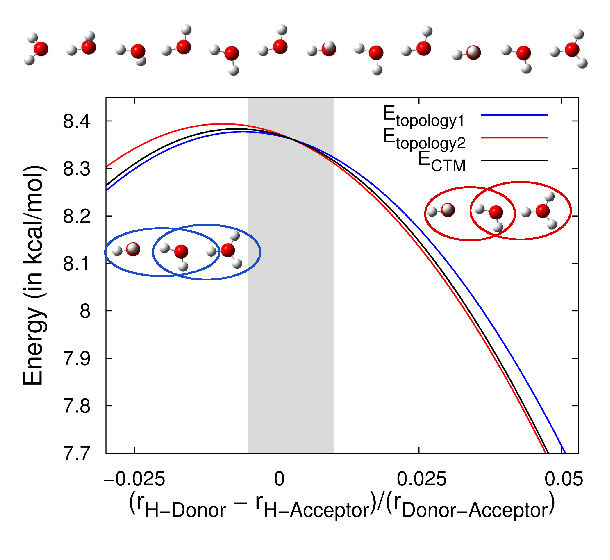
\includegraphics[width=1\textwidth]{figures/twoTopoWithWaterwireChanged.eps}
        \caption{\label{chap3fig1}}
    \end{subfigure}%
    ~
    \begin{subfigure}[t]{0.5\textwidth}
        \centering
        \includegraphics[width=1\textwidth]{figures/DiffERepeated.eps}
        \caption{\label{chap3fig2}}
    \end{subfigure}
    \caption{The potential energy surfaces corresponding to the two topologies and the interpolated
    energy are shown in Figure \ref{chap3fig1}. The difference between the
    interpolated curve and the diabatic topological curves are shown in Figure \ref{chap3fig2}.}
\end{figure*}

The interpolated PES also converges uniformly to the lower energy surfaces on both sides of the
seam. To verify this convergence of surfaces we plot the differences between the interpolated
CTM surface and the other two fragmentation topology curves in Figure \ref{chap3fig2}. As seen from Figure
\ref{chap3fig1} $E_{CTM}$ is higher than $E_{Topology1}$ on the left side and hence $E$_{CTM}-$E_{Topology1}$
should be positive on left side of the seam. This can be confirmed by Figure \ref{chap3fig2} where
the solid blue curve is positive on the left side of the seam. This same argument can also be
verified for $E_{Topology2}$ on the right side in the two figures discussed here. It can also be seen that
the difference between the CTM and the $E_{Topology1}$ is zero on the farther left of the graph and
then it has a maximum and then it decreases. The same is true for $E_{Topology2}$ if looked from the right
side instead of left.

Using all the three potential discussed above symmetrized Hamiltonians are constructed and their eigenstates are
obtained by employing Arnoldi iteration \cite{sorensen1992implicit, parlett1987complex, van1996matrix}.
Arnoldi iteration is one of the important examples of iterative methods to find eigenvalues of
general matrices. This scheme is similar to Lanczos iteration which only works for Hermitian
matrices. The ground eigenstates for CTM, topology1 and topology2 are written as $\psi_{0}^{CTM}(r)$,
$\psi_{0}^{Topology1}(r)$ and $\psi_{0}^{Topology2}(r)$ respectively.

\begin{figure}[!hbt]
  \begin{center}
    \includegraphics[width=1\textwidth]{figures/DiffEVRepeated.eps}
    \caption{\label{chap3fig3} The difference between ground state eigenvectors is plotted for the interpolated surfaces
     and the diabatic curves is plotted with respect to a modified reaction coordinate shown below the x-axis.}
  \end{center}
\end{figure}

Analogous to the comparison of difference in potentials as shown in Figure \ref{chap3fig2} we plot the corresponding
ground eigenstate differences in Figure \ref{chap3fig3}. We find that the differences in these eigenstates are
$\sim 10^{-3}$. It is however, important to note that the maximum for
$\psi_{0}^{CTM}(r)-\psi_{0}^{Topology1}(r)$ is located around the minimum of the potentials. It is due the fact that
$E_{Topology2}$ is the preferred representation chosen by $E_{CTM}$ around the minimum of these curves. Overall, these
curves show that $\psi_{0}^{CTM}(r)$ is more correlated to $\psi_{0}^{Topology1}(r)$ as compared to
$\psi_{0}^{Topology2}(r)$.

One of the future goals of this project is to also implement a topological surface-hopping
paradigm where the stochastic nature of the hop is given through a Metropolis sampling
constructed using the off-diagonal elements of the matrix $M$ discussed in the previous Chapter.
We will also analyze the formal and computational implications of a Pechukas theoretic
description of this problem. Summaries of these ideas are presented in Chapter 4.

We should emphasized the fact that in real calculations seam is not known and neither do we know
the best topology. Hence an analysis is required to see how the error in the interpolated surface behaves as a
function of different seams. This kind of analysis will tell us if a guess about the neighbourhood of
proton seam will work or not. This will specifically be very useful in the case of multi-dimensional PES
calculations, where one needs to know if a range of seam choices give similar order of accuracies. This analysis
is shown in last subsection of the next section where we present potential suface calculations for eigen cation.

\subsection{Potentials and proton eigenstates for eigen cation during dynamics}
{\label {eigenResults}}
In this section we present an analysis on the quantum nuclear effects during a classical trajectory of an eigen system.
Potential energy surfaces are important tools to study the quantum nuclear effects hence three hydrogen nuclei H1, H2
and H3 as shown in Figure \ref{eigenImage} are quantized in this study. For each of the hydrogens 1D potential surfaces
are obtained along their corresponding donor and acceptor oxygen atoms. To clarify the direction of each scan, dotted
lines passing through the hydrogens and connecting a pair of oxygens are shown in Figure \ref{eigenImage}. These
potential surfaces are calculated with initial geometries obtained at 1 ps, 2 ps and 3ps during a classical
trajectory.

\begin{figure}[H]
    \centering
    \begin{subfigure}[t]{0.5\textwidth}
        \centering
        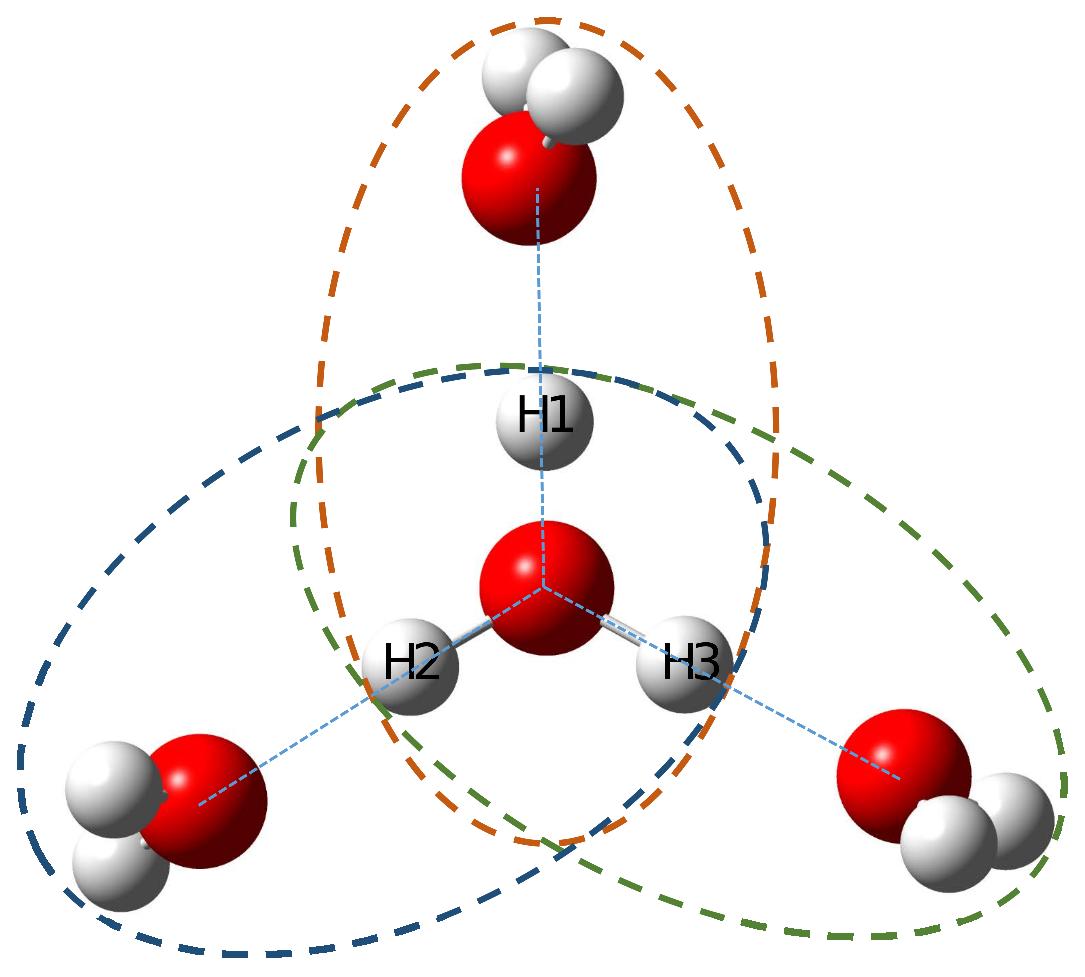
\includegraphics[width=1\textwidth]{figures/eigen1.eps}
        \caption{\label{eigenImage1}}
    \end{subfigure}%
    ~
    \begin{subfigure}[t]{0.5\textwidth}
        \centering
        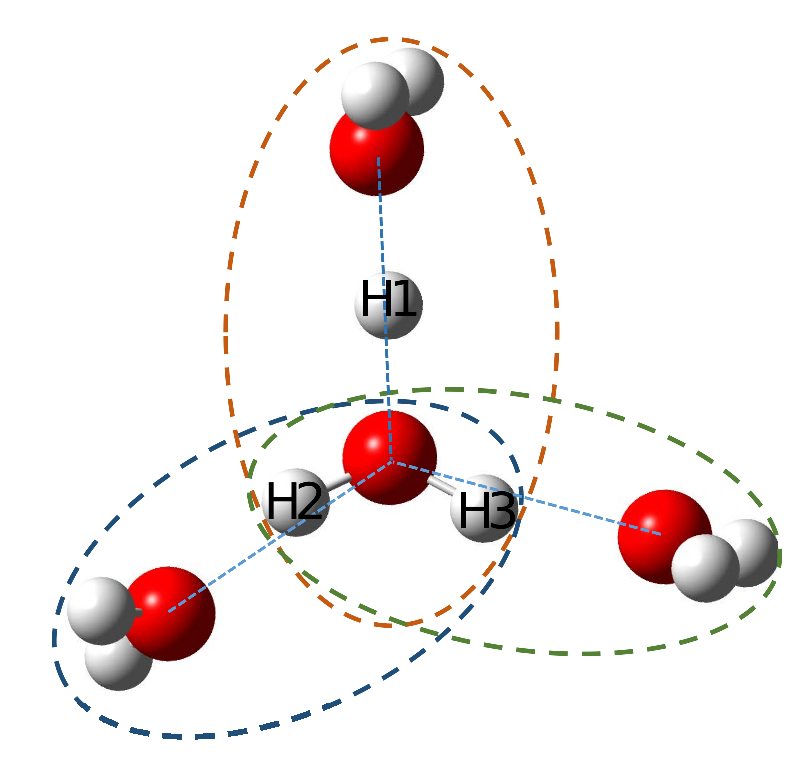
\includegraphics[width=1\textwidth]{figures/eigen2.eps}
        \caption{\label{eigenImage2}}
    \end{subfigure}
    \caption{\label{eigenImage} Figure \ref{eigenImage1} and \ref{eigenImage2} shows two of the many possible
    topologies for the potential scan of H1 along the dotted line (passing through H1) shown in the both the
    figures. Similar topologies exist for H2 and H3 for the potential scans along the dotted lines shown
    through them. The dotted lines are the vectors along their two nearest oxygen atoms.}
\end{figure}

An adaptive fragmentation scheme mentioned in Section \ref{autosubDiscussion} is utilized to obtain all the
fragment topologies during potential scans. There are a total of nine potential scans with two fragmentation
topologies in each. In figure \ref{eigenImage1} and \ref{eigenImage2} we present two of these topologies with
primary fragments shown in ellipses. Fragmentation based electronic structure calculations are done by using
PIE-ONIOM package. The user input details used in PIE-ONIOM are as shown in Table \ref{table_pieOniomDetails}
with an exception of the total number of grid points which varies due to the variation in oxygen-oxygen distances
during a classical trajectory. After the potentials are obtained for both of the topologies, those are then used
as diabatic states in the CTM program for each scan. As mentioned in Section \ref{ww12DiabaticSection}, first
ten proton eigenstates and their corresponding eigenvalues are obtained for each scan by using Arnoldi
iteration.

The accuracy of the CTM interpolation is computed as follows. The potential computed by CTM is compared with
the reference full system (MP2/6-31++g(d,p)) calculations. An estimate for the global error is computed by the
mean absolute error

\begin{equation}
\epsilon_{V} = \frac{1}{N} \sum_{i}^{}|V_{CTM}(r_{i}) - V_{MP2}(r_{i})|.
\label{meanAbsoluteError}
\end{equation}

\noindent and an estimate for cumulative error is computed by ground state weighted mean absolute error

\begin{equation}
\epsilon_{\psi_{0}} = \sum_{i} |\psi_{0}(r_{i})|^2 |V_{CTM}(r_{i}) - V_{MP2}(r_{i})|
\label{groundStateWeightedErr}
\end{equation}

\noindent between the two potential surfaces CTM and the reference.
We also compute the errors for the potentials obtained by just shifting the curves at
a particular choice of seam. We have already mentioned in Section \ref{CTMSection}
of Chapter 2 that shifting of these potential surfaces can be obtained by CTM and it is just
special case of the more general approach employed by CTM method.

\subsubsection{Error analysis on potentials obtained by CTM interpolation}
Figure \ref{chap3fig4} shows the potential surface accuracies and the ground state proton
eigenvalues for each potential surface of H1, H2 and H3. As noted in the Figure \ref{chap3fig4},
the left-vertical axis represents $\epsilon_{v}$  or $\epsilon_{\psi_{0}}$, in kcal/mol and the
right-vertical axis shows the ground state proton eigenvalues (E), in kcal/mol. The proton scans
corresponding to H1, H2 and H3 are shown for 1ps, 2ps and 3ps respectively in the x-label of the
histogram. For example, the mean absolute error $\epsilon_{v}$ of the CTM surface for H1 scan at
1ps is $\sim$ 0.14 kcal/mol and the ground state mean absolute error $\epsilon_{\psi_{0}}$ of
the surface obtained by just shifting the topologies for H2 scan at 2ps is $\sim$ 0.11 kcal/mol.
Note that $\epsilon_{\psi_{0}}$ are less than 0.14 kcal/mol for all the interpolations.

In all cases, the eigenvalue shown in Figure \ref{chap3fig4} is the lowest energy eigenvalue obtained
after Arnoldi iteration. These eigenvalues are obtained by using the reference potentials. Error
analysis on proton eigenvalues and proton eigenstates will be discussed later in this chapter.

\begin{figure}[H]
  \begin{center}
    \includegraphics[width=1\textwidth]{figures/bars.eps}
    \caption{\label{chap3fig4} Histograms shown above represent the error analysis of potential energy surfaces
    for the three protons of $H_9O_4^+$ system. The geometries used for potential energy scans are collected at
    1 ps, 2 ps and 3 ps during the dynamics. Scans are done using fragment based electronic structure methods
    CTM and JS. The results are compared with full system mp2 calculations for the corresponding potential
    energy scans. $\epsilon_{V}$ and $\epsilon_{\psi_{0}}$ are the errors defined by equation 1 and 2
    respectively. Eigenvalues corresponding the ground state of each potential are plotted in the right y-axis.}
  \end{center}
\end{figure}

\subsubsection{Potential and ground state analysis during a classical dynamics trajectory}
$\bf{I~ have~ not~ re-written~ this~ subsection}$

For all the potential scans of eigen cation discussed above, potential and their proton ground states
($\Psi_{0}$) are shown in Figure \ref{chap3fig5}. Red curves shown in Figure \ref{chap3fig5}
correspond to the potentials and the blue curves correspond to $\Psi_{0}$. By looking at Figure
\ref{chap3fig5} we can analyze the quantum nature of the hydrogen nucleus at different times
during dynamics simulation. The delocalization of these three eigenstates can be seen from the
location of their peaks and their spread along x-axis. For H1, initially at 1 ps the ground state
is peaked at around 0.3 on x-axis and it moved to around 0.75 at 2 ps. This means that proton
moved towards acceptor $H_2O$ molecule and got stabilized. This stabilization is clearly visible
from the clear single well shape of the potential shown at 2 ps as compared to almost a double well
potential at 1 ps. But the proton again moved back towards donor to around 0.55 at 3 ps. As the
proton was already in a stable position, not much change in the shape of potentials can be
observed from 2 ps to 3 ps for H1. As the wavefunction has the same sign throughout x-axis,
it highest peak also corresponds to the point of highest probability. Similarly, for H2, the
proton moved towards acceptor atom by a small amount during 1 ps to 2 ps. H2 again remained in a
stable situation from 2 to 3 ps. The shapes among all three protons can be compared depending
on their location of peaks. It can be seen that only two of the three protons show any kind
of double well character at any instant of time. At 1 ps, H3 is in most stable state, at 2 ps
H1 is the most stable among all and at 3 ps also H1 remained the most stable. This kept the
other two potentials to remain in a similar shape.

\begin{figure}[H]
  \begin{center}
    \includegraphics[width=1\textwidth]{figures/E.eps}
    \caption{\label{chap3fig5} Figure shows potentials V(r)(in red) and ground states \(\Psi_{0}\) (in blue) for
    $H_9O_4^+$ system for geometries collected at 1 ps, 2 ps and 3 ps during dynamics. X-axis is the difference
    of the distance between the proton and the donor Oxygen atom and the proton and the acceptor Oxygen atom
    in each case.}
  \end{center}
\end{figure}

To make sure that CTM captures the quantum mechanical nature of protons H1, H2 and H3 in an accurate way,
we do an error analysis on first ten proton eigenstates and eigenvalues for H1, H2 and H3 in the next sub-section.

\subsubsection{Accuracy of proton eigenstates and eigenvalues obtained by CTM}
Quantum mechanical nature of protons is represented by the eigenfunctions and eigenvalues of their Hamiltonian.
Hydrogen nucleus being light shows quantum mechanical behavior in proton transfer reactions. To capture these
effects such as tunnelling and zero point effects, we must have accurate eigenfunctions. 

Figure \ref{chap3fig6} shows the accuracy of first ten proton eigenstates and their corresponding eigenvalues
obtained by using CTM potentials, individual topology potentials and their shifted case (shown by JS) for the
proton
scans discussed above in the eigen system. To clarify the notations, Topology1 and Topology2 correspond
to the errors obtained by using only one topology at a time. As noted in each case, the left-vertical axis represents
$L_{2}$ norm of the error in eigenfunctions, $\epsilon_{\Psi_{i}}$ for all i $\in$ \{0, 1 , ... ,9\} and is scaled
by $10^5$. On the other hand the right-vertical axis shows the $L_{2}$ norm of the errors in their corresponding
eigenvalues, in kcal/mol and is scaled by 10. Different potentials employed in this error analysis are mentioned in
the figure legend. For example, the $L_{2}$ norm of the error in the eigenfunction $\epsilon_{\Psi_{0}}$ for the H2
scan at 1ps obtained by using CTM potential surface is $\sim 5\times10^{-5}$ and the $L_{2}$ norm of the error in the
eigenfunction $\epsilon_{\Psi_{7}}$ for the H1 scan at 2 ps obtained by using Topology1 potential surface is
$\sim 19.5 \times10^{-5}$. Note that the errors in the CTM case are less than $8\times10^{-5}$ in most of the proton
eigenstates. Although some of the topology errors are less than CTM in specific cases, such as the error in
$\epsilon_{\Psi_{3}}$ for the H1 scan at 2 ps is lower for Topology2 as compared to its CTM error. But non of the two
topologies are consistent with their trends in error and we would not know which topology to choose to get those
accuracies. Hence, an optimal method which gives consistently good results should be employed.

In all cases, the errors in eigenvalues shown by $\epsilon_{E}$ correspond to the eigenvalues of the same
eigenfunction as mentioned on the left-vertical axis. The $L_{2}$ norm of the error in the eigenvalues are
less than 0.1 kcal/mol for the lower eigenstates such as $\Psi_{0}$, $\Psi_{1}$,$\Psi_{2}$,$\Psi_{3}$. It
can be noted from the right side of the figure that $\epsilon_{E}$ increases for higher eigenstates but is
still under 0.3 kcal/mol. Upon further inspection of \ref{chap3fig6}, it follows that the errors of eigenfunctions
as well as eigenvalues vary simultaneously in almost all the cases presented here. For example, $\epsilon_{\Psi_{4}}$
and the corresponding $\epsilon_{E}$ both have a sharp peak for H1 scan at 2ps obtained by Topology1.

\begin{figure}[H]
  \begin{center}
    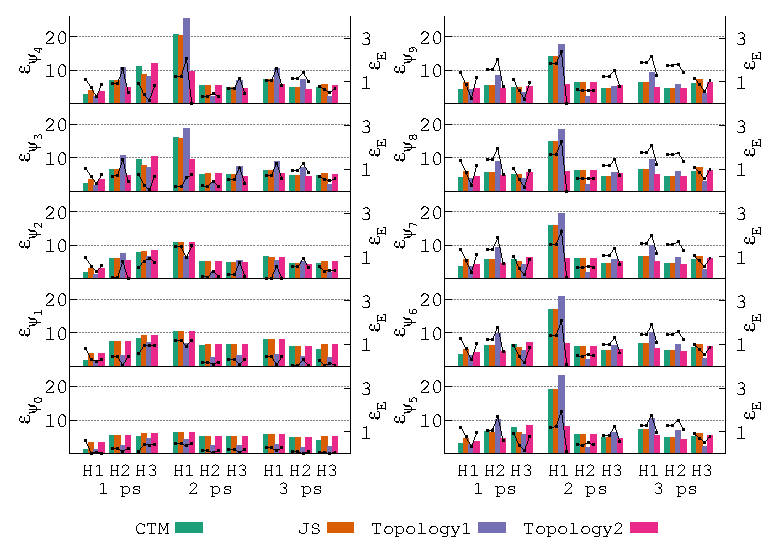
\includegraphics[width=1\textwidth]{figures/eigenEvalEditted.eps}
    \caption{\label{chap3fig6} Figure shows the L2 norm errors in first ten proton eigenstates(on left axis) and
    the corresponding eigenvalues(on right axis, in kcal/mol) for $H_9O_4^+$. The error in eigenstates is scaled
    by a factor of $10^5$ and the errors in eigenvalues are scaled by 10.}
  \end{center}
\end{figure}

We discussed at the end of Section \ref{ww12DiabaticSection}, that dependence of error on the choice of seam
needs attention and should be rigorously studied. In next subsection we present an analysis on errors in CTM as a
function of seams.

\subsection{Potential surfaces for water-wire systems}
{\label {waterwireResults}}
As mentioned previously in Section \ref{intoToTestSystems} protonated waterwires are known to play important
roles in many processes in biological membranes, fuel cell, nanotubes etc.  In all these processes, quantum
nature of protons play a crucial role in the outcome of the process. For example proton tunneling is know to
increase the rate of many proton transfer reactions.
We analyze three waterwire systems in this section out of which $(H_{2}O)_{12}H^+$ has already been introduced
in the Section \ref{ww12DiabaticSection} and the other two waterwires $(H_{2}O)_5H^+$ and $(H_{2}O)_3H^+$
are smaller versions of $(H_{2}O)_{12}H^+$. In all the three waterwires, we calculate reduced dimensional
potential scans to analyze quantum nature of the extra proton in these linear chains of water molecules. To
obtain the potential energies with the post Hartree-Fock accuracy at the cost of DFT, we employ fragment
based electronic structure calculations with the help of PIE-ONIOM package on a grid.
Topologies are generated by the adaptive fragmentation scheme mentioned in Section
\ref{autosubDiscussion}. Diabtic state curves are obtained by utilizing these fragment topologies in
PIE-ONIOM package. User input details used in PIE-ONIOM vary in each case. For $(H_{2}O)_{12}H^+$, we calculate
two potential surfaces by scanning H1 and H2 shown in Figure \ref{waterwiresFigure} along their nearest Oxygen
atoms. PIE-ONIOM user inputs for these two potentials are same as the details mentioned in Table \ref{table_pieOniomDetails}
except the number of grid points and number of topologies in H2 case. On the other hand, for $(H_{2}O)_5H^+$ and
$(H_{2}O)_3H^+$ protons scans are done for H1 atoms (shown in Figure \ref{waterwiresFigure}) only but are done
with two different Higher level of theories MP2/6-31++g(d,p) and CCSD/6-31++g(d,p) respectively.

\begin{figure}[H]
    \begin{subfigure}[t]{0.29\textwidth}
        \includegraphics[width=0.9\textwidth]{figures/ex3ww.eps}
        \caption{\label{ex3ww}}
    \end{subfigure}%
    ~
    \begin{subfigure}[t]{0.6\textwidth}
        \hfill\includegraphics[width=0.9\textwidth]{figures/ex5ww.eps}
        \caption{\label{ex5ww}}
    \end{subfigure}
    ~
    \begin{subfigure}[t]{0.29\textwidth}
        \includegraphics[width=0.9\textwidth]{figures/in3ww.eps}
        \caption{\label{in3ww}}
    \end{subfigure}%
    ~
    \centering
    \begin{subfigure}[t]{0.6\textwidth}
        \hfill\includegraphics[width=0.9\textwidth]{figures/in5ww.eps}
        \caption{\label{in5ww}}
    \end{subfigure}
    ~
    \centering
    \begin{subfigure}[t]{0.99\textwidth}
        \includegraphics[width=0.99\textwidth]{figures/ex12ww.eps}
        \caption{\label{ex12ww}}
    \end{subfigure}
    ~
    \centering
    \begin{subfigure}[t]{0.99\textwidth}
        \includegraphics[width=0.99\textwidth]{figures/in12ww.eps}
        \caption{\label{in12ww}}
    \end{subfigure}
    \caption{\label{waterwireImage} In the above Figure, the pair of Subfigures $\{a,c\}$, $\{b,d\}$ and $\{e,f\}$
    represent the two topologies for the waterwires $(H_{2}O)_{3}H^+$, $(H_{2}O)_{5}H^+$ and $(H_{2}O)_{12}H^+$
    respectively. Blue and red ellipses represent the primary fragments corresponding to two different topologies
    and the darkest ellipse represents the changing primary fragment in each case. The dotted black line passing
    through a hydrogen atom represents the direction of proton scan in each Subfigure.}
\end{figure}


After we obtain these diabatic potential energy curves, we interpolate them using CTM program and compare the
surface with full system calculations done at their corresponding higher level of theories.
In next, we show the accuracy the error analysis for of CTM surfaces.

\subsubsection{Accuracy of CTM interpolated potentials for waterwires}
The errors in CTM interpolated potential surfaces are calculated as $\epsilon_{V}$ and $\epsilon_{\psi_{0}}$
defined by Eq. \ref{meanAbsoluteError} and Eq. \ref{groundStateWeightedErr} respectively. Figure \ref{chap3fig7}
shows the errors $\epsilon_{V}$ and $\epsilon_{\psi_{0}}$ along with the ground state
proton eigenvalues of various potential scans of three waterwires. The left-vertical axis represents the error in
the CTM potentials, in kcal/mol, and the right vertical axis shows the ground state proton eigenvalues obtained
by using the reference full system potentials, in kcal/mol. The details about molecular system corresponding to
each proton scan is written right below the horizonal axis labels. For example 12 ww, 5 ww and 3 ww represent
$(H_{2}O)_{12}H^+$, $(H_{2}O)_{5}H^+$ and $(H_{2}O)_{3}H^+$ respectively. The labels ``mp2'' and ``ccsd'' mean
that the Higher level of theory in the Fragment based electronic structure calculations are MP2 and CCSD
respectively. Note that $\epsilon_{\psi_{0}}$ is always less than $\epsilon_{V}$ and all the ground state
weighted CTM errors are less than 0.1 kcal/mol. The peaks corresponding to CTM interpolation errors for H2 scan
of 12 ww and H1 scan of 5 ww seem like outliers but their ground state weighted versions suggest that the regions
containing most of the error in potential have less probability of wavefunction. It also turn out to be a case
in these specific potential scans that the errors of CTM match exactly with JS in most of the cases.

In all cases, the ground state proton eigenvalues are shown by square dots and their magnitudes correspond
to the right-vertical axis. For example the ground state eigenvalue for H1 for 12 ww is higher than H2, this
means that the potential corresponding to H2 is broader than the potential corresponding to H1. This also
means that H1 is bound strongly to one of the oxygens as compared to H2. In case of 5 ww and 3 ww, the
groundstate eigenvalues corresponding to CCSD are lower than the ones corresponding to their MP2 potentials
which means that the CCSD potentials are broader for H1 scans in both the cases as compared to their MP2 scans.

We need to see how the proton ground state looks like for the interpolated potentials. This gives us an insight
on what is the probability that the hydrogen is delocalised across the grid. In next subsection we present
all the interpolated potentials with their ground eigenstates calculated in this study of waterwires.

\begin{figure}[H]
  \begin{center}
    \includegraphics[width=1\textwidth]{figures/wwbars.eps}
    \caption{\label{chap3fig7} Histograms shown above represent the error analysis of potential energy surfaces
    for the three different protonated water-wire structures $(H_{2}O)_{12}H^+$, $(H_{2}O)_5H^+$ and $(H_{2}O)_3H^+$
    respectively. Potential energy scans are calculated for two protons H1 and H2 for $(H_{2}O)_{12}H^+$. For
    both $(H_{2}O)_5H^+$ and $(H_{2}O)_3H^+$ potential energy scan are calculated for proton H1. All the
    calculations are done using fragment based calculations and the higher level of theory for each case is
    mentioned below the histograms. The results are compared with higher level full system calculations for the
    corresponding potential energy scans. $\epsilon_{V}$ and $\epsilon_{\psi_{0}}$ are the errors defined by
    equation 1 and 2 respectively. Eigenvalues corresponding the ground state of each potential are plotted
    in the right y-axis.}
  \end{center}
\end{figure}

\subsubsection{CTM interpolated potentials and corresponding proton ground states}
To see the delocalization of quantized protons, we observe their ground eigenstates and see how far from
their classical location do they seen non-zero. If the proton is more delocalised then is shows more
quantum effects for example in case of tunneling the proton eigenstate would be delocalised across the barrier.

Figure \ref{chap3fig8} shows the CTM interpolated potentials and proton ground eigenstates for $(H_{2}O)_{12}H^+$,
$(H_{2}O)_5H^+$ and $(H_{2}O)_3H^+$ respectively. The left-vertical axis shows the magnitude of potential (V(r)),
in kcal/mol and the right-vertical axis shows the magnitude of the corresponding proton ground eigenstates
($\Psi_{0}$). The details about to proton and the molecular system are mentioned on top of each graph. For
example, the red curve shown on the left-bottom side of the Figure \ref{chap3fig8} shows the potential surface for
H2 in $(H_{2}O)_{12}H^+$ system. The blue curve in the same plot shows the proton ground eigenstate obtained
by using its CTM potential. Note that the maximum of eigenvectors are located at the minimum of their potentials.
This is just mean that the hydrogen nuclei have maximum probability of their existence in the neighborhood of
their classical location. All except one (H1 scan of $(H_{2}O)_{12}H^+$) of the potentials look more like a double well rather than single well potentials. This also follows from the rate at which eigenstate decay in their
potentials. For example, H1 scan calculated with MP2 as higher level for $(H_{2}O)_{5}H^+$ shows enhanced
delocalization as compared to H1 of $(H_{2}O)_{12}H^+$ which decays exponentially. In fact, we should expect
quantum tunneling through the barrier in case of H1 scan calculated with MP2 as higher level for
$(H_{2}O)_{5}H^+$. In fact, H2 scan of $(H_{2}O)_{12}H^+$ as well as H1 scan of $(H_{2}O)_{3}H^+$ calculated using
MP2 as higher level also show some non-zero probability on the other side of the barrier.

\begin{figure}[H]
  \begin{center}
    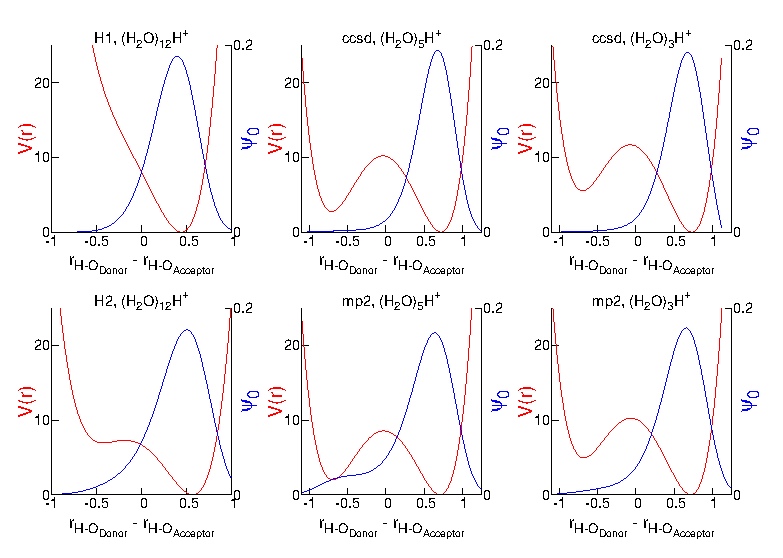
\includegraphics[width=1\textwidth]{figures/wwE.eps}
    \caption{\label{chap3fig8} Figure shows potentials V(r)(in red) and ground states \(\Psi_{0}\) (in blue)
    for the three different protonated water-wire structures $(H_{2}O)_{12}H^+$, $(H_{2}O)_5H^+$  and
    $(H_{2}O)_3H^+$ respectively. The x-axis is the difference of the distance between the proton from the
    donor Oxygen atom and the proton from the acceptor Oxygen atom in each case.}
  \end{center}
\end{figure}

Other than just focussing on the potentials and proton ground states, we need to see how accurate are the
excited states for protons are after calculating through CTM potentials. In next section we look into the
accuracy of first ten proton eigenstates and eigenvalues corresponding to each of the proton scans shown
for these three waterwires.

\subsubsection{Accuracy of proton eigenstates and eigenvalues for waterwires}
We calculate $L_{2}$ norm of the errors in proton eigenstates and see how well are they
represented by CTM interpolation. We also calculate these errors for the special case of CTM interpolation
discussed in Section \ref{CTMSection} which turn out to be shifting of diabatic states. Other than these we
look into errors in proton eigenvectors obtained from individual topologies and compare them to the CTM
results.

Figure \ref{chap3fig9} shows errors in proton eigenstates and the corresponding eigenvalues for CTM,
special case of CTM(JS) and the individual topologies. As noted in each case, the left-vertical axis
represents the $L_{2}$ norm of the errors in eigenstates and is scaled by $10^{4}$. On the other hand,
the right-vertical axis shows the error in the calculation of the corresponding proton eigenvalues, in
kcal/mol and is scaled by 10. The histograms stacked on top of each other correspond to the same proton
scan and same systems. The information about the protons and their level of theories is given right
below the horizontal axis. For example, all the dark green peaks on the left most side of all the histograms
correspond to the H1 scan of $(H_{2}O)_{12}H^+$. Note that the errors in the ground eigenstate are the lowest
ones as compared to other eigenstates. This trend is similar to the eigen cation case shown in previous section
in Figure \ref{chap3fig6}. In all the cases, there exist at least one topology which performs worse than CTM
interpolation. In some of the cases, there exist a topology which performs equally well or even better than
CTM but again, we would not know this choice of topology in the general case. Overall, the errors in the CTM
case are consistently low than the individual topologies.

In all cases, the errors in CTM proton eigenstates are relatively better than other methods. For example,
CTM is the only case whose errors in the proton eigenvalues are on the lower side of the available errors.
Although the errors in the ground state are relatively low in all the cases but the difference can observed
in the higher eigenvalues. The error in CTM proton eigenvalues is still lower than 0.25 kcal/mol in all the
cases.

%Error analysis for first ten proton eigenstates and the corresponding eigenvalues is also done for all water-wire
%potentials discussed above. This analysis is shown in figure \ref{chap3fig9} where the height (shown on the left
%y-axis) of the bars represent the errors in eigenstates and their magnitude is multiplied by a factor of $10^4$.
%Similarly, the errors in the eigenvalues are represented (on right y-axis) by squares dots and but their
%magnitude is scaled by 10. As it can be seen that eigenstates are well represented by all the methods and
%the errors for eigenstates is less than $6\times 10^{-4}$ in all the cases. On the other hand the errors in
%the eigenvalues are all less than 0.6 kcal/mol and most of the CTM errors are even less than 0.2 kcal/mol. 

\begin{figure}[H]
  \begin{center}
    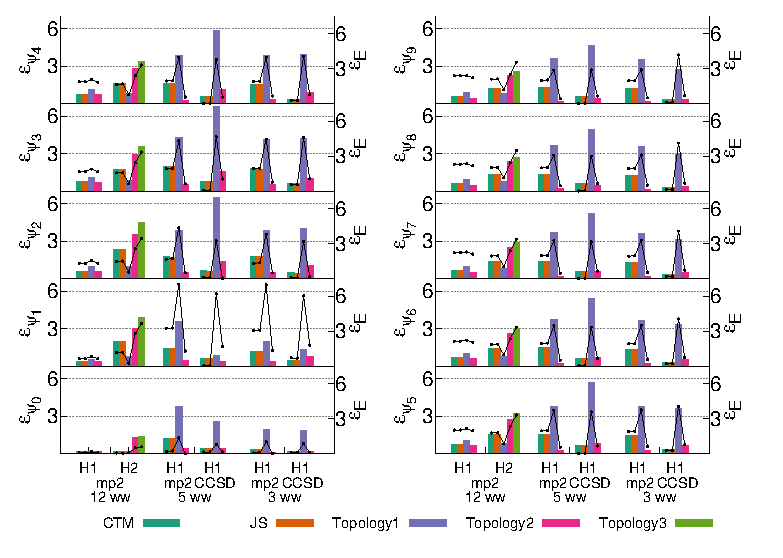
\includegraphics[width=1\textwidth]{figures/barsEditted.eps}
    \caption{\label{chap3fig9} Figure shows the L2 norm errors in first ten proton eigenstates(on left axis) and
    the corresponding eigenvalues(on right axis, in kcal/mol) for three different protonated water-wire structures
    $(H_{2}O)_{12}H^+$, $(H_{2}O)_5H^+$ and $(H_{2}O)_3H^+$. The errors in proton eigenstates are scaled by a
    factor of $10^4$ and the errors in eigenvalues are scaled by 10.}
  \end{center}
\end{figure}

As it can be observed clearly that H2 scan of $(H_{2}O)_{12}H^+$ is the only case studied until now which
involved more than two diabatic surfaces. It would interesting to look more closely in the CTM interpolation
for this 3 by 3 case of interpolation. In next subsection we present details of the CTM interpolation of
this special case.

\subsubsection{CTM interpolation using three diabatic states in waterwires}
Any problem in fragment based potential surfaces or dynamics which involves three topologies is an good platform
for algorithms designed to solve N-topology problems. We utilize this opportunity to see how well our program
works on real three topology problems. We start with a grid on which we want to create the potential surface
calculations and we utilize an adaptive topology generation scheme described in Section \ref{autosubDiscussion}.
We then obtain three different topologies within our grid points. Then we utilize PIE-ONIOM to obtain potential
curves corresponding to each of these three topologies. These three potential curves are then used as diabatic
input curves to CTM program and we obtain an interpolated CTM surface.

Figure \ref{chap3fig10} consists of two different graphs. The lower graph shows three diabatic surfaces and
their CTM interpolated surface. On the other hand, the upper graph describes the differences between the
interpolated curve and the individual topologies. The boxes have been drawn on the lower graph to show the
enhanced version of these surfaces. It should be noted that the order of these curves change in the subsequent
boxes which is a proof of their intersections. The points shown by dotted vertical lines on the horizontal axis
are in fact the points chosen as seam inputs in CTM program. The pink curve is shown to be in between
the other two curves in the left most box. In the right most box, it is shown that the CTM curves is lowest in
energy.

To get clearer picture of the behavior of interpolated curve with respect to the individual topology curves,
we need to see the difference between the interpolated surface with the topology surfaces. It can be seen from
the upper curve that the CTM curve is equal to Topology1 on the left most side and then it smoothly switches to
Topology2 and finally to Topology3 curves on the right side of the shown picture. Hence the interpolation works
well for three topology cases as well.

%A close analysis on the H2 PES for $(H_{2}O)_{12}H^+$ is done to show the accuracy of the method for more than two
%topology cases. This analysis is shown graphically by Figure \ref{chap3fig10} which shows two graphs in on one below
%the other. The lower graph shows four potential energy surfaces (three for the fragmentation topologies and one for 
%CTM. Due to their closeness rectangles are drawn on the these PES as an attempt to show their differences from each
%other. Although, only three of the four PES are visible even after zooming in. Hence, the difference between CTM and
%the fragmentation topologies PES are plotted on the curve shown on top. This can be seen that CTM is equal to
%topology3 on the left side and then it switches to topology2. The topology 2 then finally switches to topology1
%on the right side. The two seams are shown by plotting two dotted perpendicular lines from the intersection
%of curves to the x-axis. The details of the PES at these seams are also shown by two of the rectangles in
%the lower graph. The zoomed in version of the left rectangle show that the PES corresponding to topology2 and
%topology3 intersect and they are clear lower in energy from topology1 by around 0.1 kcal/mol. The zoomed in version
%of the rectangle in the middle shows that topology3 is higher in energy than other curves which is clear from the top
%graph as at this point the topology2 switches to topology3. Other than these two seams the minimum is also
%analyzed by zooming in a rectangle. This shows that these curves are shifted to match at those respective seams
%and they don't have the same minimum. In fact the topology1 PES is lowest among the topology curves which can
%also be seen by the top graph as the difference between CTM and topology1 is zero on the right side.
%)
\begin{figure}[H]
  \begin{center}
    \includegraphics[width=1\textwidth, trim= 0 1 0 0, clip=true]{figures/threeTopoCase.eps}
    \caption{\label{chap3fig10} Figure shows PES and difference between CTM and others for a $3 \times 3 $ case.
    Lower graph shows the PES for three fragmentation topologies and the CTM interpolated potential. The rectangles
    are drawn to show zoomed in version of different portions of the graph. The upper graph shows the differences
    between the CTM and other fragmentation topology potentials.}
  \end{center}
\end{figure}

We now are interested in testing the CTM interpolation in higher order problems. In the next section
we utilize analytical potentials and see how CTM works on those surfaces.

\section{Unknown seam}
{\unknownSeamSection}

\subsection{Error in CTM interpolation as a function of seams}
Due to the lack of knowledge about the exact locations of seams, we need to guess a ``small'' neighborhood
around them. If we are close to the ``real'' seam, then we can expect the CTM interpolation to work fine
but the question remains, how big can that neighborhood be? We begin with this thought process and assume a finite
neighborhood. Then we calculate errors in CTM interpolation as a function of each of the points in that neighbourhood.

\begin{figure}[htb!]
  \begin{center}
    \includegraphics[width=1\textwidth]{figures/autosubScanEigen.eps}
    \caption{\label{autosubScanEigen} Figure shown above represents the error analysis of potential energy (on the
    left) and the proton ground states (on the right) as a function of different seams for the three
    centre most hydrogens of $H_9O_4^+$ system. The geometries used for potential energy scans are the same as
    discussed in this same section. Potential Scans are done using fragment based electronic
    structure methods CTM and JS. The results are compared with full system mp2 calculations and $\epsilon_{V}$
    and $\epsilon_{\psi_{0}}$ are the errors defined by Eq. \ref{meanAbsoluteError} and
    Eq. \ref{groundStateWeightedErr} respectively. The error on the left axis is scaled by 10 and the on the
    right axis is scaled by 10000.
    }
  \end{center}
\end{figure}

Figure \ref{autosubScanEigen} shows $L_{2}$ norm of the errors for CTM potential surfaces and their corresponding
proton ground eigenstates with full system MP2/6-31++g(d,p) as the reference calculation in the eigen system scans
described earlier in this section. As noted in each case, the left-vertical axis represents error in CTM potentials
($\Delta V$), in kcal/mol and is scaled by 10. On the other hand, the right-vertical axis represents error in the
proton ground eigenstates ($\Delta \psi_{o}$). The parameter on horizontal axis varies with the choice of seams and
is calculated in the same way as the horizontal axis parameters shown in Figure \ref{chap3fig5}. The two
curves $\Delta V^{CTM}$ and $\Delta V^{JS}$ shown for each proton scan correspond to the $L_{2}$ norms of errors
in potential for CTM interpolation and its special case of shifting the curves respectively. In five out of nine
potential scans the two curves CTM and JS match almost exactly but there are variation in the others. The maximum
variation in the CTM potential surface errors for the choice seam in this neighborhood varies from scan
to scan but it is still less than 0.06 kcal/mol in all the cases. This means that the exact location of seam doesn't
play important role in the interpolation. An approximate guess for the seam can be used as
input to CTM program to get the interpolated surface.

In all the cases, the where the errors for potential between CTM and JS match almost exactly, their errors in
proton ground eigenstates also match closely. Although the maximum variation in the proton ground eigenstate is
$\sim 10^{-4}$, but for most of the cases errors are still of the order of $10^{-6}$.

After completing the analysis on eigen cation system, we move on to the other class of protonated water cluster
we talked earlier. In next section we apply CTM interpolation on different potential surface calculations of
waterwire systems.
 

\begin{figure}[htb!]
  \begin{center}
    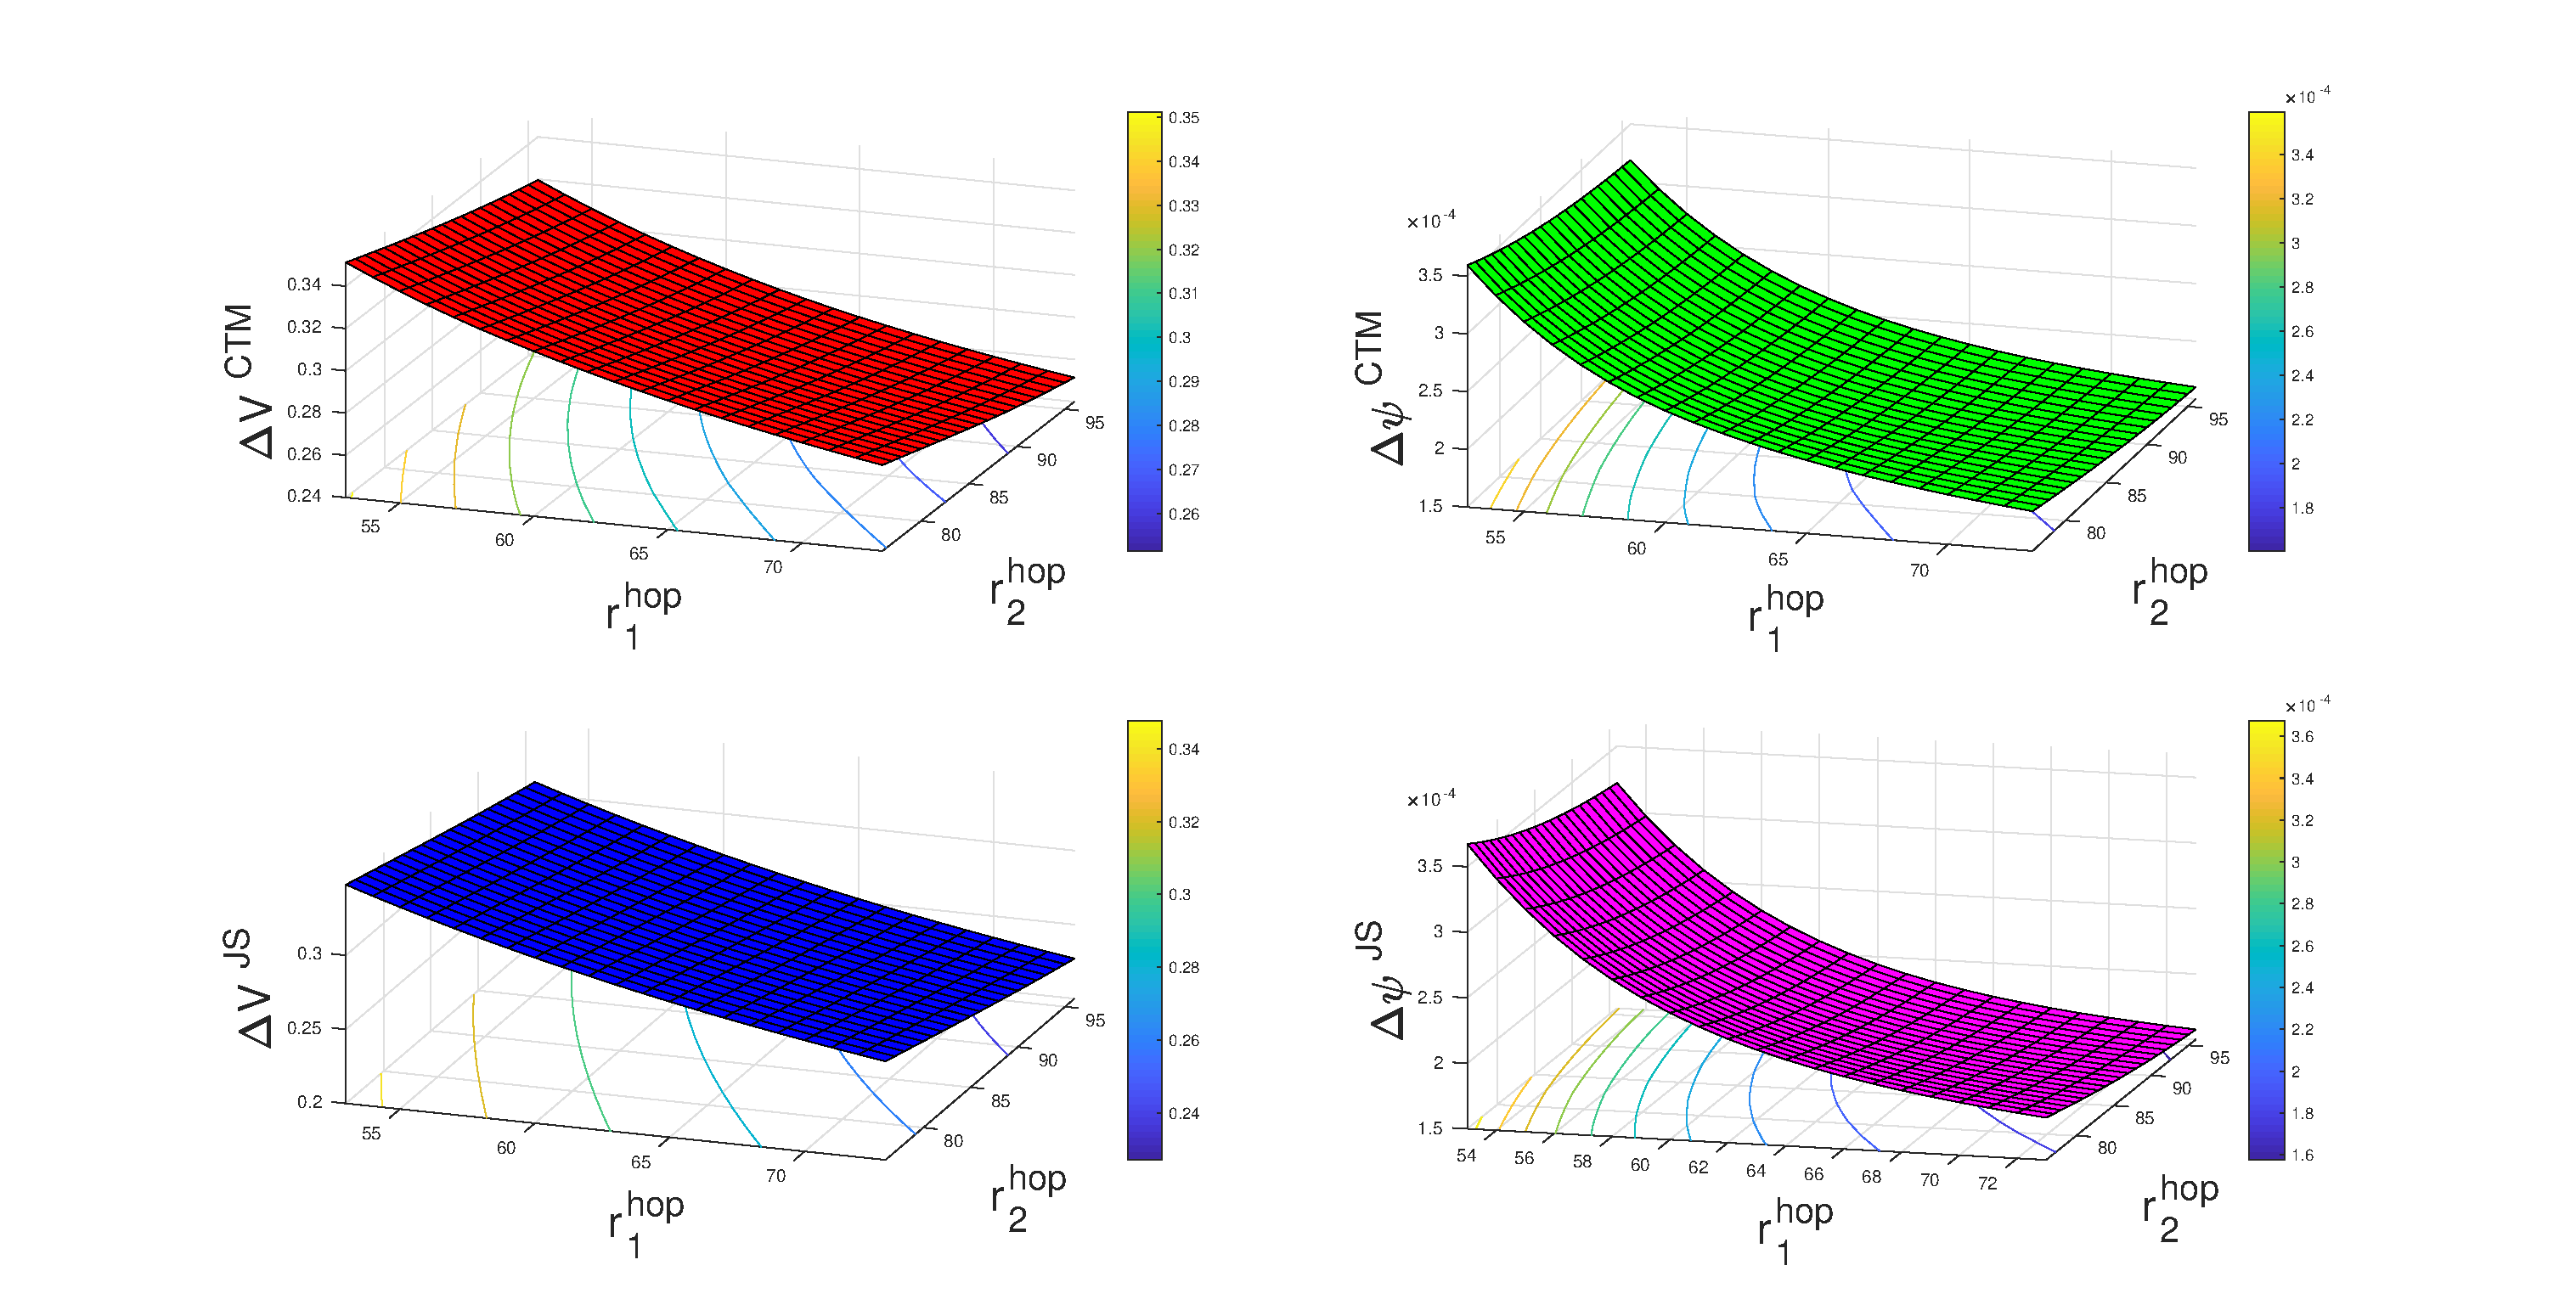
\includegraphics[width=1\textwidth]{figures/autosubError.eps}
    \caption{\label{autosubScanEigen} Figure shown above represents the error analysis of potential energy (on the
    }
  \end{center}
\end{figure}





\section{Coupled proton motion}
{\label {analyticalPotentials}}
Let us see, how this interpolation works for some analytical functions. Let,
$V_{1}(x)$, $V_{2}(x)$, $V_{3}(x)$ and $V_{4}(x)$ be polynomials representing four potential energy
curves along a reaction coordinate $x$. These polynomials are given by:
\begin{eqnarray*}
V_{1}(x) = (x - 1)x^{3} \\
V_{2}(x) = (x - 2)x^{3} \\
V_{3}(x) = (x - 3)x^{3} \\
V_{4}(x) = (x - 4)x^{3}
\end{eqnarray*}

We can see that this is a case of 4 by 4 CTM interpolation. These curves along with their CTM
interpolated curve are shown in Figure \ref{4by4PES}. It can seen from Figure \ref{4by4PES} that the
curves intersect at $x_{12}$, $x_{23}$ and $x_{34}$ and hence these are the seams.

\begin{figure*}[hbt!]
    \centering
    \begin{subfigure}[t]{0.5\textwidth}
        \centering
        \includegraphics[width=1\textwidth]{figures/potentialsGraph.eps}
        \caption{\label{4by4PES}}
    \end{subfigure}%
    ~
    \begin{subfigure}[t]{0.5\textwidth}
        \centering
        \includegraphics[width=1\textwidth]{figures/diffGraph.eps}
        \caption{\label{4by4Diff}}
    \end{subfigure}
    \caption{Potential surfaces for analytical functions $V_{1}(x)$, $V_{2}(x)$, $V_{3}(x)$ and
    $V_{4}(x)$ are shown in Figure \ref{4by4PES}. Difference between the CTM interpolated curve
    and the individual analytical functions is shown in Figure \ref{4by4Diff}.}
\end{figure*}

The potential energy value for the CTM curve matches exactly with the respective intersecting
curves at $x_{12}$, $x_{23}$ and $x_{34}$. It can also be seen that the CTM curve is always close
to the lowest curve among all the polynomial curves but is never lower than all. The behaviour of
interpolation can be analyzed more clearly by plotting the difference of interpolated CTM curve and
the polynomial curves with coordinate axis $x$. These difference plots are shown in Figure
\ref{4by4Diff}. It can be seen from Figure \ref{4by4Diff} that the difference between $V_{1}(x)$ and
CTM curve goes to zero on far left of the coordinate axes. Similarly the difference between
$V_{4}(x)$ and CTM curve goes to zero on far right of the coordinate axis $x$.
The CTM interpolated curve transitions from $V_{1}(x)$ to $V_{2}(x)$ at $x_{12}$. On the left of
$x_{12}$, CTM curve starts to deviate from $V_{1}(x)$ but then comes back to it, exactly at $x_{12}$.
The same behaviour is shown for the transition from $V_{2}(x)$ to $V_{3}(x)$ at $x_{23}$ and
$V_{3}(x)$ to $V_{4}(x)$ at $x_{34}$ respectively. It can also be observed that there are some small
jumps in the CTM graph close to the point where the differences become zero. These jumps are due to the
truncation of error function in the neighbourhood of seams. These neighbourhoods are user
defined and can be adjusted to have a low truncation error. Beyond these neighbourhood, CTM program
chooses the lowest curve among all the available curves.

\newpage

